\chapter{Investigation on the Most Forward Going Events}
\label{app:forward_investigation}

This appendix focuses on some effect that may affect the data/simulation discrepancy observed in the most forward going bins in the $\cos\theta$ distribution, Figure~\ref{fig:trkcostheta_xsec}.

One possible cause may be due in the mis-modelling of the kaon flux, as kaons are responsible for producing high energy neutrinos, that are mostly forward going. 
%To study this, the cross section as a function of $\cos\theta$ was extracted with and without a cut on the reconstructed muon momentum at 2.5 GeV in both data and \acrshort{mc}. This is shown in Figure \ref{fig:xsec_2_5cut}. The plots show the nominal cross section (black) with statistical and systematic errors bars. The red curve shows the central value result for the sample that includes the momentum cut. The only visible difference is in the most forward going bin and it is negligibly small compared to our error bars.
%
%
%\begin{figure}[t]
%%\begin{adjustwidth}{-1cm}{-1cm}
%\centering
%\subfloat[][]
%   {\includegraphics[width=.45\textwidth]{images/MomentumCut2_5/xsec_mumom_2_5cut}
%   \label{fig:xsec_mumom_2_5cut}} \quad
%\subfloat[][]
%   {\includegraphics[width=.45\textwidth]{images/MomentumCut2_5/xsec_muangle_2_5cut}
%   \label{fig:xsec_muangle_2_5cut}} \\
%\caption{Data extracted cross section as a function of reconstructed muon momentum and angle. Black is nominal, red is with an additional cut in the events section that requires all events to have reconstructed momentum smaller than 2.5 GeV.}
%\label{fig:xsec_2_5cut}
%%\end{adjustwidth}
%\end{figure}
The kaon contribution of the neutrino flux was studied. The plot in Figure \ref{fig:kaonscaled} shows the event distributions after background subtraction and efficiency correction (not cross sections) as a function of reconstructed muon momentum and muon angle for Tune 1, Tune 3, and data. For Tune 1, the events with a kaon parent were weighted 50\% up and down to illustrate the effect on the event distributions. This change affects most strongly the forward going bin. A change of 50\% in the kaon flux contribution over all energies results in a change that is still smaller than the total error bars, and smaller than the difference between Tune 1 and Tune 3.

\begin{figure}[t]
%\begin{adjustwidth}{-1cm}{-1cm}
\centering
\subfloat[][]
   {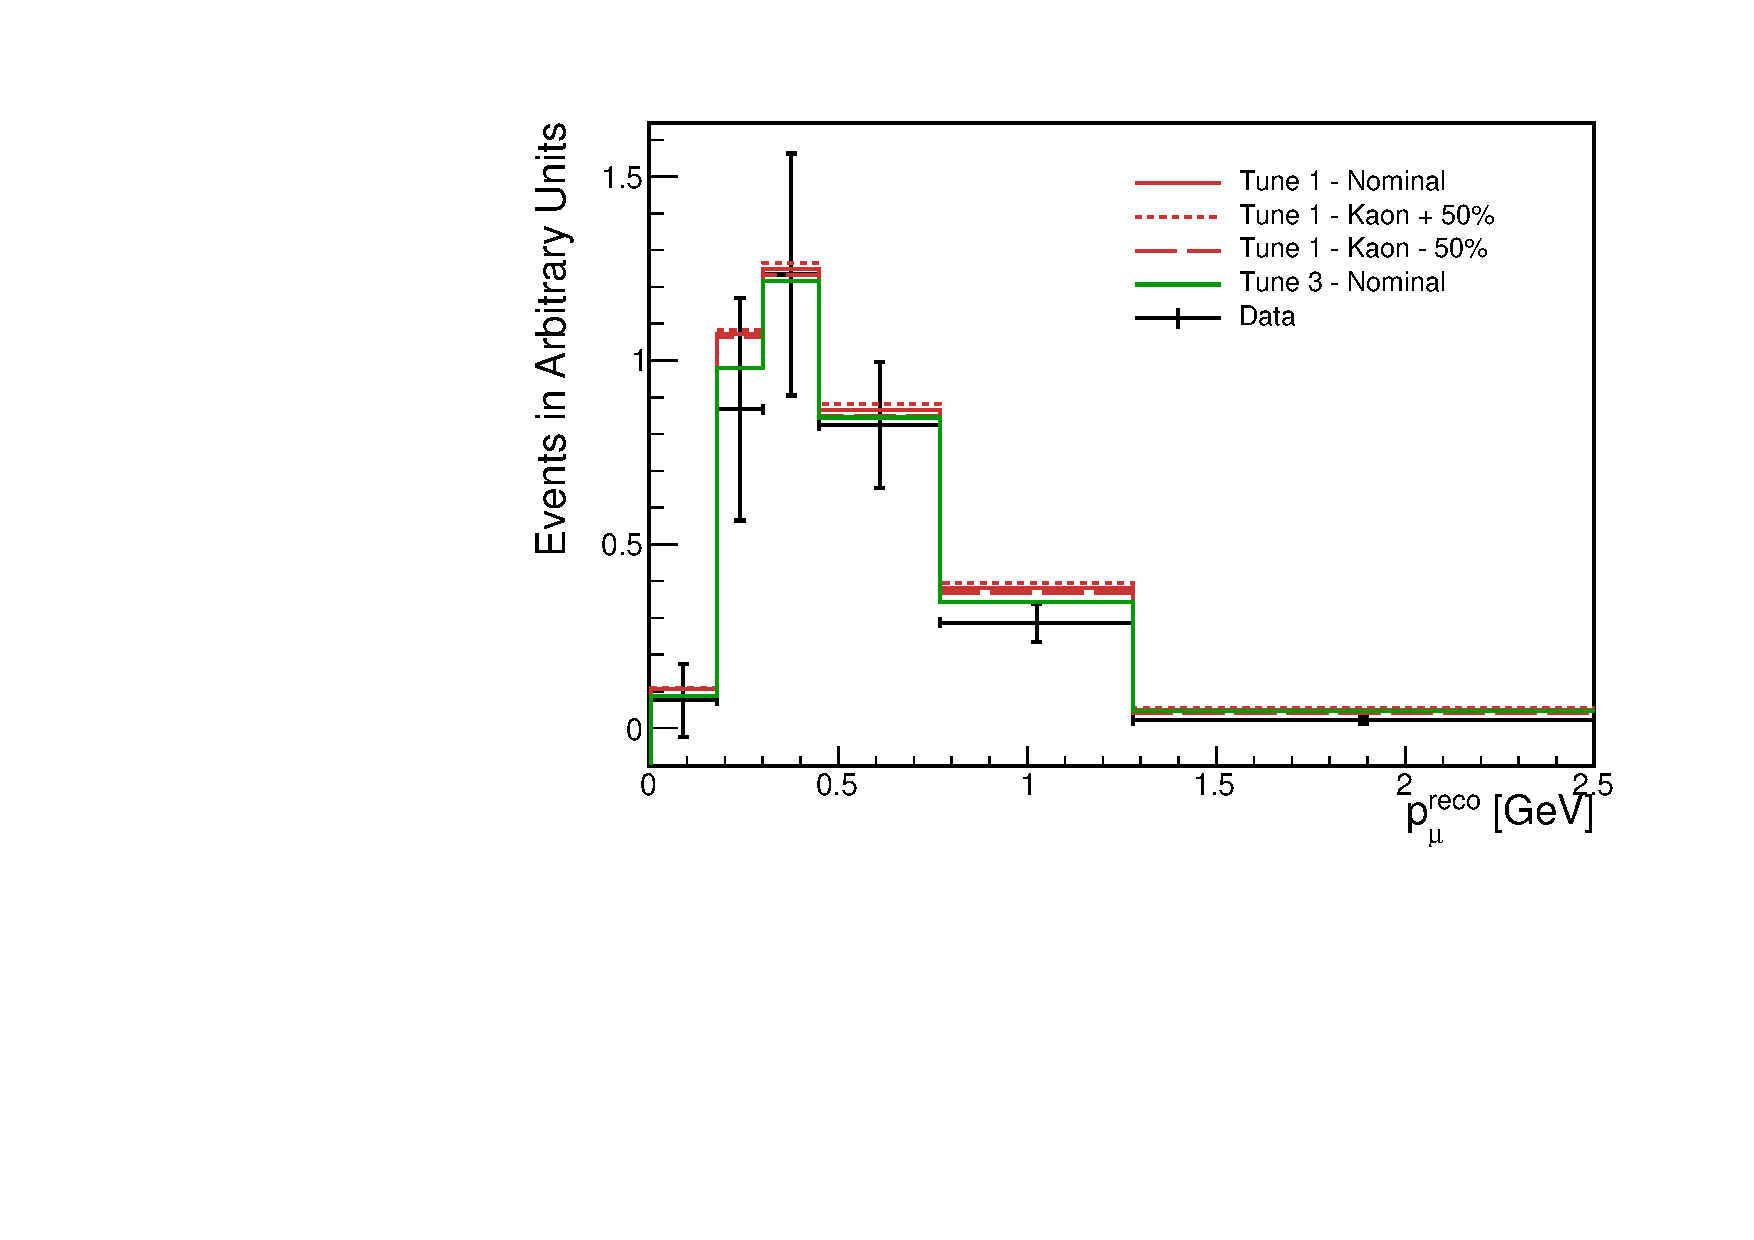
\includegraphics[width=.45\textwidth]{images/KaonScaled/events_mumom_kaonscaled}
   \label{fig:events_mumom_kaonscaled}} \quad
\subfloat[][]
   {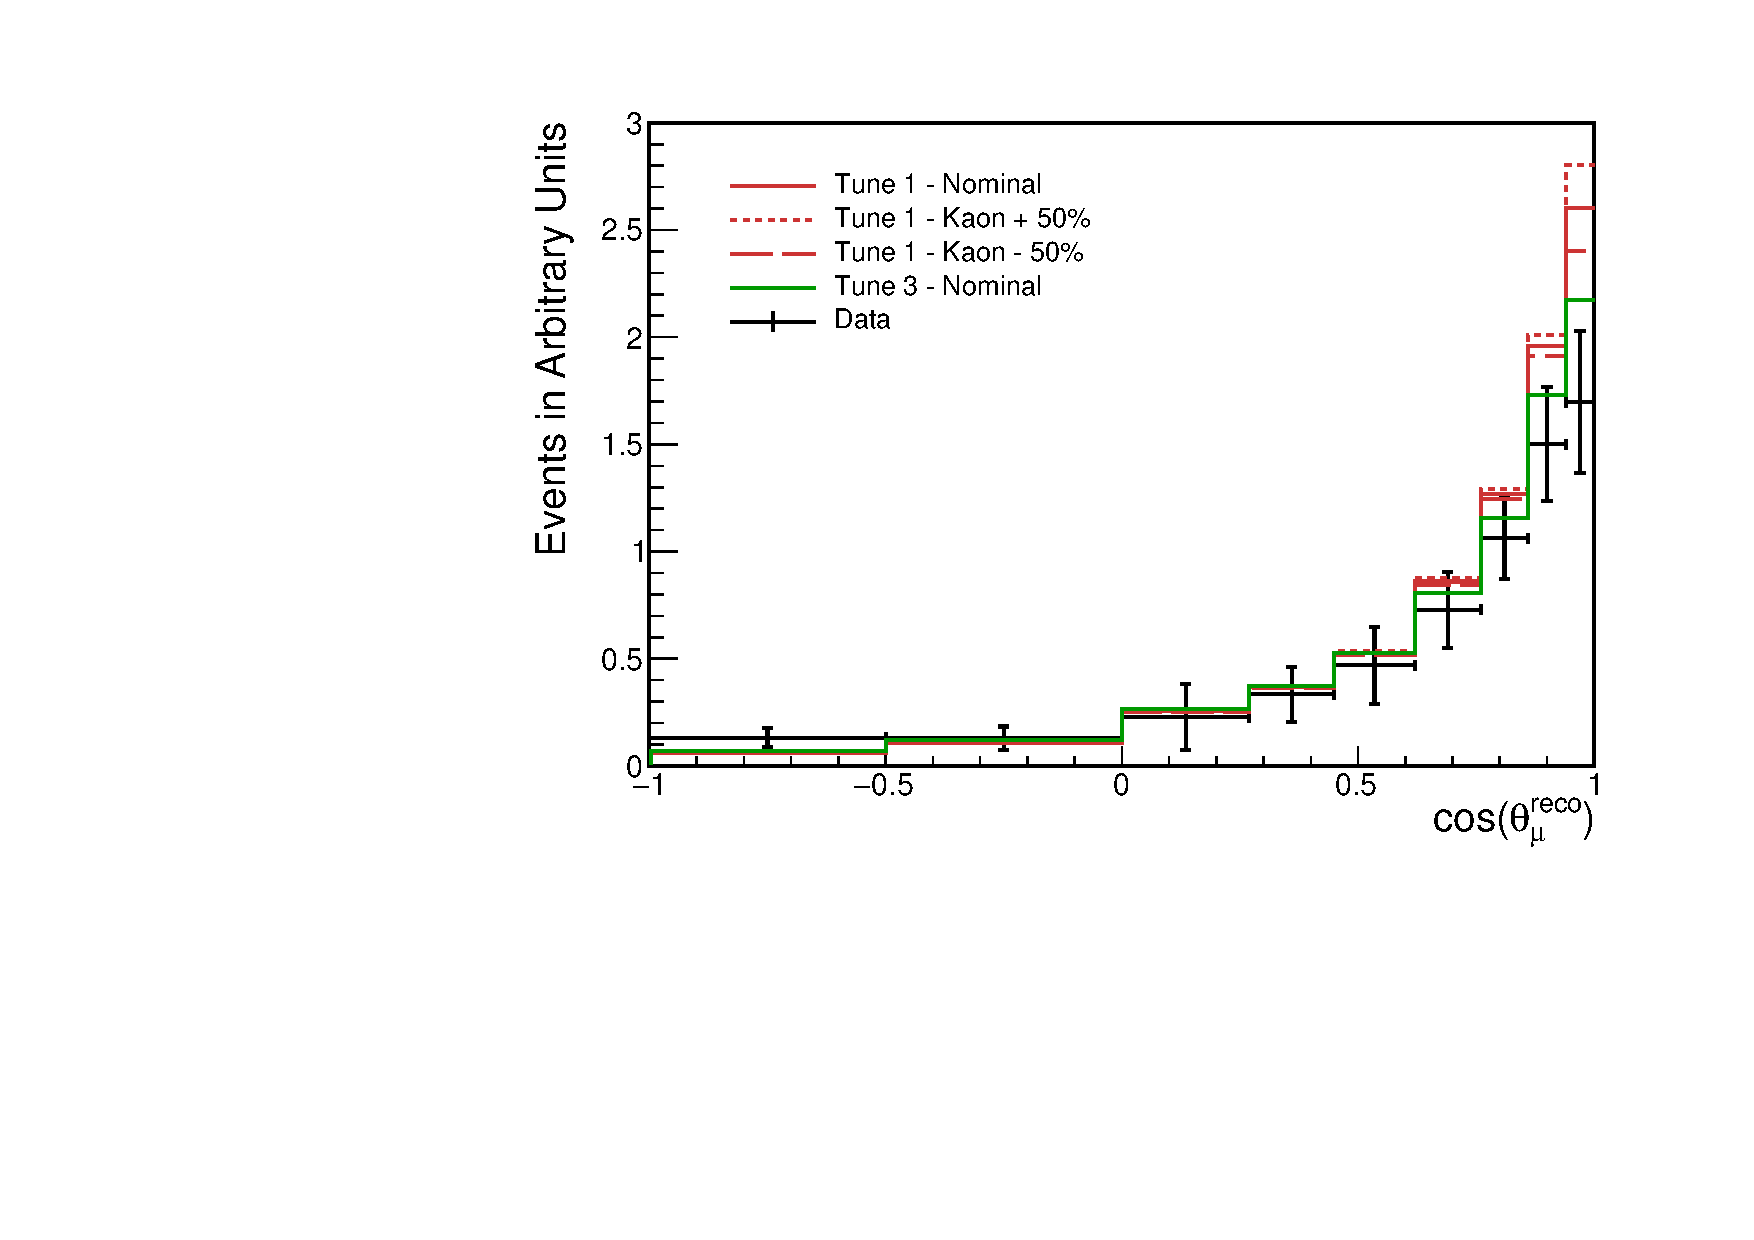
\includegraphics[width=.45\textwidth]{images/KaonScaled/events_muangle_kaonscaled}
   \label{fig:events_muangle_kaonscaled}} \\
\caption[Event Distributions with Kaon Flux Scaled]{Number of events (in arbitrary units) for \acrshort{mc} Tune 1 nominal (red solid), and \acrshort{mc} Tune 3 nominal (green), and data (black). The kaon flux was scaled by $\pm$ 50\% in Tune 1 \acrshort{mc} (red dashed and dotted lines).}
\label{fig:kaonscaled}
%\end{adjustwidth}
\end{figure}


One other issue may be due to the discrepancy in the $\phi$ distribution, Figure~\ref{fig:trkphi_tune1}. 
Figure \ref{fig:xsec_phicuts} shows the cross section as a function of $\cos\theta_\mu$ for four different regions of phi: 4 quadrants to select upwards, downwards, anode-pointing and cathode-pointing tracks. The black curve is the nominal cross section with statistical and systematic error bars, and the different colours are the central values for each quadrant of phi, respectively. The total uncertainty covers all central value results.

\begin{figure}[]
\centering
\includegraphics[width=.50\textwidth]{images/PhiCuts/xsec_muangle_phicuts}
\caption[Cross Section in Different $\phi$ Quadrants]{Black shows the nominal cross section. Coloured lines show the cross section selecting 4 different quadrants in $\phi$.}
\label{fig:xsec_phicuts}
\end{figure}

